
\section{Conclusi�n}
\begin{frame}{Conclusi�n}

\framesubtitle{Logros}

\end{frame}
%
\begin{frame}[shrink]{Conclusi�n}

\framesubtitle{Trabajos Futuros}

\setbeamercovered{transparent}
\begin{columns}[t]

\column{0.6\textwidth}
\begin{itemize}[<+->]
\item Segmentar en grupos para modelos espec�ficos.
\item Incorporar en \emph{\structure{\emph{HARDroid}}} otros m�todos de
aprendizaje. 
\item Incluir m�s variables que mejoren el clasificador.
\item Extender \emph{\structure{\emph{HARDroid}}} para identificar m�s
actividades en otros contextos. 
\item Experimentar con accesorios que incluyan se�ales relevantes. 
\end{itemize}

\column{0.4\textwidth}
\begin{overprint}
\onslide<1> 
\begin{center}
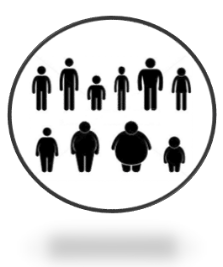
\includegraphics[width=0.8\textwidth]{conclusion/graphics/groups}
\par\end{center}

\emph{\footnotesize{}Rangos de edad, sexo y/o factores fisiol�gicos}{\footnotesize \par}
\onslide<2> 

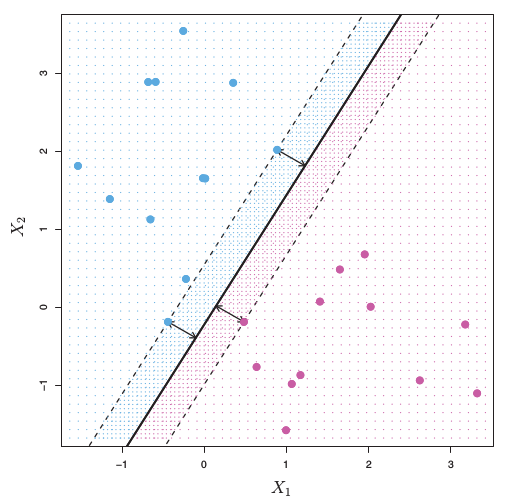
\includegraphics[width=1\textwidth]{conclusion/graphics/svm}

\emph{\footnotesize{}Explorar m�todos SVM (Support Vector Machine)
o ANN (Artificial Neural Networks)}{\footnotesize \par}
\onslide<3> 

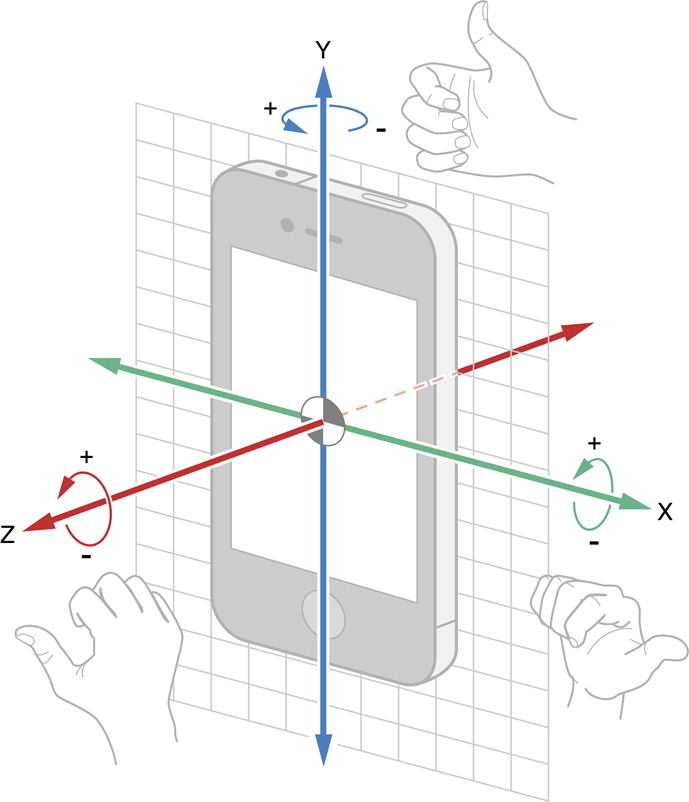
\includegraphics[width=1\textwidth]{conclusion/graphics/gyro}

\emph{\footnotesize{}Orientaci�n del dispositivo}{\footnotesize \par}
\onslide<4> 
\begin{center}
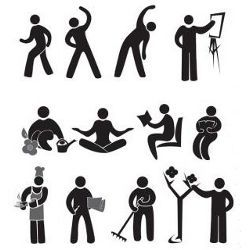
\includegraphics[width=1\textwidth]{conclusion/graphics/activities}
\par\end{center}

\begin{center}
\emph{\footnotesize{}Acciones diarias}
\par\end{center}{\footnotesize \par}
\onslide<5> 
\begin{center}
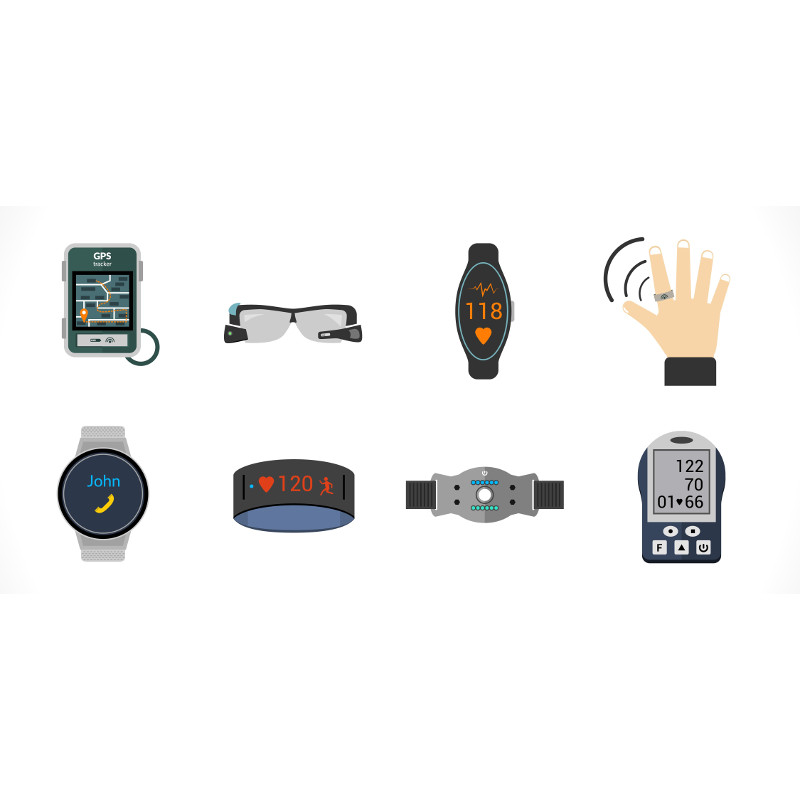
\includegraphics[width=1\textwidth]{conclusion/graphics/wear}
\par\end{center}

\emph{\footnotesize{}Accesorios como Smartwatch, Smartband, entre
otros}{\footnotesize \par}
\end{overprint}
\end{columns}

\end{frame}
%
\begin{frame}
\begin{center}

\includegraphics[width=0.8\textwidth]{conclusion/graphics/thanks}
\par\end{center}

\begin{center}
\structure{\begin{center}
por su atenci�n!!!
\par\end{center}}
\par\end{center}
\end{frame}

